\section*{Problem 4: Multiple Choice [5 pts]} 

\def\layersep{2.5cm}

\begin{enumerate}[noitemsep]
    \begin{figure}[H]
    \centering
    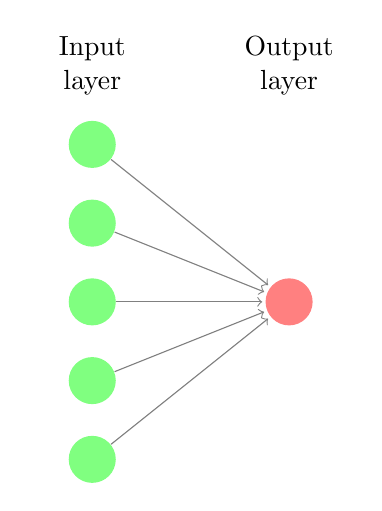
\begin{tikzpicture}[shorten >=1pt,->,draw=black!50, node distance=\layersep]
        \tikzstyle{neuron}=[circle,fill=black!25,minimum size=17pt,inner sep=0pt]
        \tikzstyle{input neuron}=[neuron, fill=green!50];
        \tikzstyle{output neuron}=[neuron, fill=red!50];
        \tikzstyle{annot} = [text width=4em, text centered]
        \foreach \name / \y in {1,...,5}
            \node[input neuron] (I-\name) at (0,-\y) {};
        \node[output neuron, right of=I-3] (O) {};
        \foreach \source in {1,...,5}
            \path (I-\source) edge (O);
        \node[annot,above of=I-1, node distance=1cm] (il) {Input layer};
        \node[annot,right of=il] {Output layer};
    \end{tikzpicture}
    \end{figure}
    \item \textbf{[1 pt]} What is the most common name of the neural network shown in the figure above, when sigmoid activation functions are being used?
    \begin{enumerate}
        \item Perceptron
        \item Kernel Regression
        \item Logistic Regression
        \item Capsule Network
    \end{enumerate}

    \begin{soln}
        % Type solution here
    \end{soln}

    
    \hfill \linebreak
    
    \item \textbf{[1 pts]} What does the decision boundary of the neural network shown in the figure above look like when sigmoid activation functions are being used?
    \begin{enumerate}
        \item Logistic
        \item Quadratic
        \item Linear
        \item Non-linear
    \end{enumerate}

    \begin{soln}
        % Type solution here
    \end{soln}

     \pagebreak
     
    \begin{figure}[H]
    \centering
    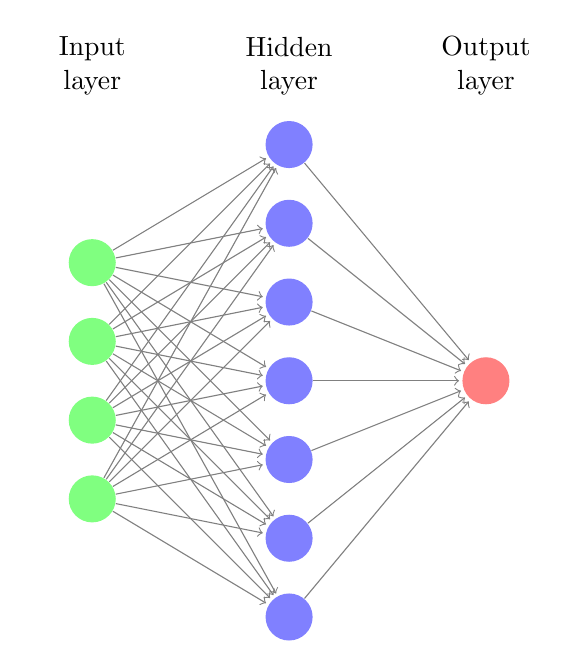
\begin{tikzpicture}[shorten >=1pt,->,draw=black!50, node distance=\layersep]
        \tikzstyle{neuron}=[circle,fill=black!25,minimum size=17pt,inner sep=0pt]
        \tikzstyle{input neuron}=[neuron, fill=green!50];
        \tikzstyle{output neuron}=[neuron, fill=red!50];
        \tikzstyle{hidden neuron}=[neuron, fill=blue!50];
        \tikzstyle{annot} = [text width=4em, text centered]
        \foreach \name / \y in {1,...,4}
            \node[input neuron] (I-\name) at (0,-\y) {};
        \foreach \name / \y in {1,...,7}
            \path[yshift=1.5cm]
                node[hidden neuron] (H-\name) at (\layersep,-\y cm) {};
        \node[output neuron, right of=H-4] (O) {};
        \foreach \source in {1,...,4}
            \foreach \dest in {1,...,7}
                \path (I-\source) edge (H-\dest);
        \foreach \source in {1,...,7}
            \path (H-\source) edge (O);
        \node[annot,above of=H-1, node distance=1cm] (hl) {Hidden layer};
        \node[annot,left of=hl] {Input layer};
        \node[annot,right of=hl] {Output layer};
    \end{tikzpicture}
    \end{figure}
    
    \item \textbf{[2 pts]} Now consider the model shown in the figure above, instead of the previous one. Why might this be a better model?
    \begin{enumerate}
        \item It has a faster training and inference time than that of a linear model.
        \item It requires less space in memory to store model parameters when compared to logistic regression.
        \item It learns a non-linear decision boundary.
        \item It will underfit to the data, making it easy to train with less data.
    \end{enumerate}

    \begin{soln}
        % Type solution here
    \end{soln}
    
    \hfill \linebreak
    \item \textbf{[1 pts]} We use hinge loss a surrogate loss for 0/1 loss, because hinge loss is:
    \begin{enumerate}
        \item Convex and differentiable
        \item Differentiable but not convex
        \item Convex but not differentiable 
        \item Neither convex nor differentiable 
    \end{enumerate}

    \begin{soln}
        % Type solution here
    \end{soln}
    
\end{enumerate}



